\chapter{TIMING ANALYSIS}
\label{chap:timing}

%%%%%%%%%%%%%%%%%%%%%%%%%%%%%%%%%%%%%%%%%%%%%%%%%%%%%%%%%%%%%%%%%%%%%%%%%%%%%%%

\section{Packet detection}

Timing analysis is used to determine the point in time where the packet starts.
This is also a method to recognize \emph{whether} a packet has arrived or not.
In the current scheme, the packet detection module uses the Schmidl and Cox %(TODO: Put citation here)
method for timing analysis.

This entire section will assume a level of abstraction wherein we have an
inexhaustible data source of digital, complex symbols at the receiver. We
acquire this data by reading from this source into a buffer (which is simply an
array) in our receiver program's source code.

\subsection{The Schmidl and Cox algorithm}

For the receiver to be able to pick out a packet from ambient noise and
interference, the transmitted packet must be designed for detection. All
transmitted packets have a \emph{preamble}, which consists of two identical
halves. Each half is a pseudo-random-number sequence. The correlation of each
half with with other (independent and hence uncorrelated) signals is expected
to be low. However, its correlation with the other half will be high. Moreover,
this property is well-maintained even when the preamble is passed through an
ISI channel with additive white gaussian noise.

In other words, we can detect the start of a packet by correlating two adjacent
windows, each having half the size of the preamble, with each other. The point
where this correlation value becomes high can be taken to be the start of the
packet.

\begin{figure}[h]
	\centering
	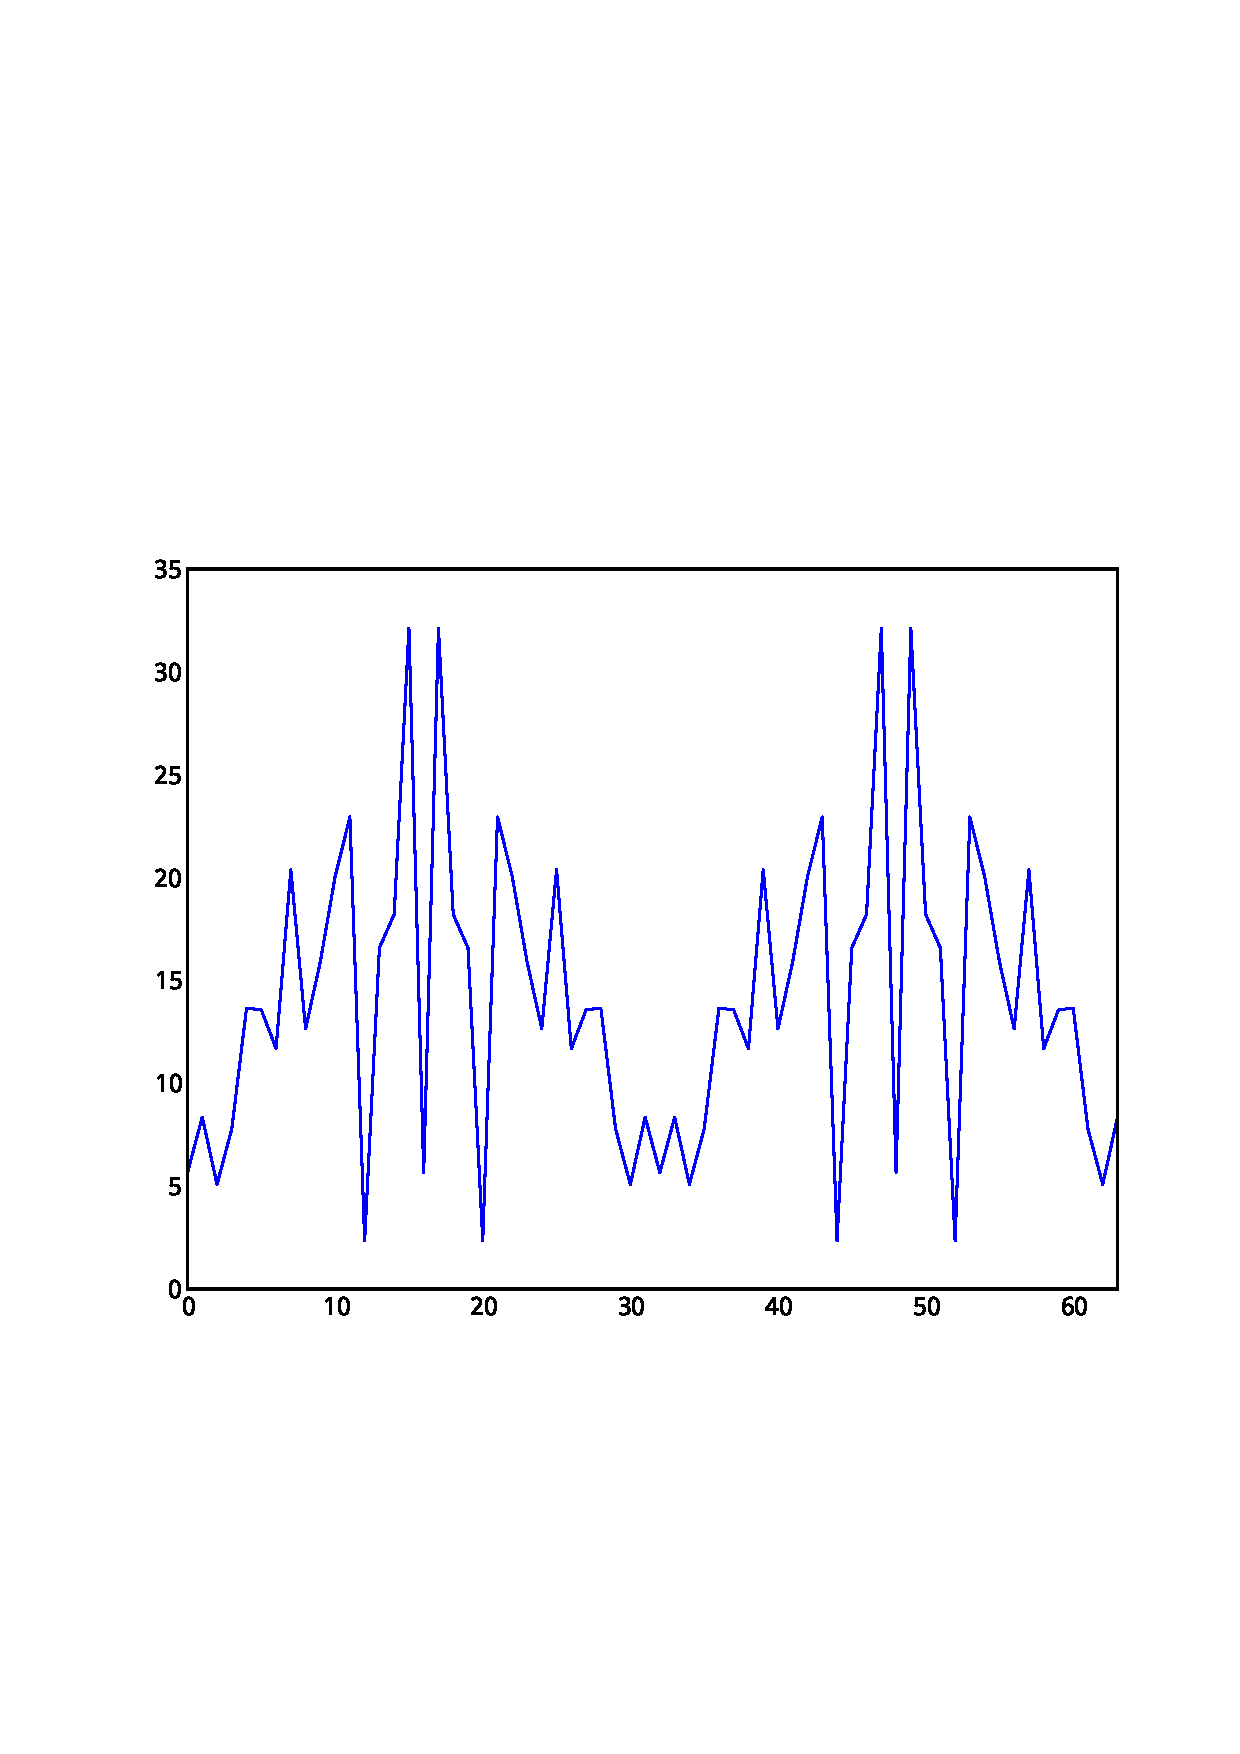
\includegraphics[width=0.8\textwidth]{preamble-abs}
	\caption{Absolute value of the preamble}
	\label{fig:preamble-abs}
\end{figure}

The metric used to determine whether or not the correlation value is high
enough is the normalized cross-correlation, defined as
$$ \text{Metric} = \frac{|\text{ Cross-correlation of the two windows }|}
                        {\sqrt\text{Product of the autocorrelations of the
                                    windows}}
$$
Let $\ue{x}$ be the vector of complex values corresponding to the first window
and $\ue{y}$ be that corresponding to the second. Then, the metric $m$ is
given by
\begin{equation} \label{eqn:old-metric}
	m = \frac{|\corr{\ue{x}}{\ue{y}}|}{|\ue{x}||\ue{y}|}
\end{equation}
where $(^*)$ denotes complex conjugation in the case of scalars and complex
conjugate transpose in the case of vectors. All vectors are taken to be row
vectors.

% TODO: Insert a picture of the metric over the data

\subsection{Running correlation on the receive buffer}

In order to efficiently perform a running correlation of adjacent windows over
an entire receive buffer, we minimize the number of computations performed. On
moving one step, we add the latest correlation point and subtract the oldest
correlation point.

\begin{figure}[h]
	\centering
	\includegraphics[width=0.8\textwidth]{correlation-windows}
	\caption{Correlation windows}
	\label{fig:corr-win}
\end{figure}

Let $\{x_i\}_{i=0}^{n-1}$ and $\{y_i\}_{i=0}^{n-1}$ be complex sequences
corresponding to the symbols in the left window and the right window
respectively, where $n$ is the window size, which is half the length of the
preamble. In the next time step, these windows are denoted as
$\{x_i\}_{i=1}^{n}$ and $\{y_i\}_{i=1}^{n}$ respectively.\footnote{Note that
for the purpose of these calculations, the two windows may be disconnected or
overlapping. No assumptions are made regarding the equality of certain ranges
of $x_i$ and $y_i$. Specifically, we do \emph{not} assume that $x_n = y_0$.
Thus, when $x_i = y_i\;\forall\;i\in\{0,1,\ldots n-1\}$, we automatically
arrive at the running autocorrelation formula.}

Let $c_{old}$ be the correlation of windows in the current time step, and
$c_{new}$ be the correlation of the windows in the next time step. That is,
\begin{equation}
	c_{old} = \sum_{i=0}^{n-1}{\corr{x_i}{y_i}}
\end{equation}
\begin{equation}
	c_{new} = \sum_{i=1}^n{\corr{x_i}{y_i}}
\end{equation}
We can then write $c_{new}$ in terms of $c_{old}$ as follows:
\begin{align}
	c_{new} &= \sum_{i=0}^{n-1}{\corr{x_i}{y_i}} - \corr{x_0}{y_0}
	                                             + \corr{x_n}{y_n} \\
	        &= c_{old} - \corr{x_0}{y_0} + \corr{x_n}{y_n}
	                                                     \label{eqn:old-update}
\end{align}

This way, once we have acquired the correlation of the first $n$ symbols, the
correlation of subsequent windows is an $\mathcal{O}(1)$ process.

\subsection{Implementation using the two-frame block}
\label{subsec:two-frame-impl}

In order to implement the Schmidl and Cox algorithm, we need to continuously
scan through the received symbols, correlating two windows, each half the size
of the preamble. Once the preamble is found, we need to pull out a full
\verb+frame_size+ number of symbols from the buffer.

Obviously, the receive buffer should be at least as long as the preamble. But
if the receive buffer is too long, then depending upon the rate of
communication, we may be adding latency to our program by having to wait for
the buffer to get filled. If our receive buffer is only one \verb+frame_size+
long, then on finding the preamble in the middle of this buffer, we will have
to take into account how many symbols more we need to extract for the frame
from the next buffer. This is cumbersome and error-prone.

\begin{figure}[h]
	\centering
	\includegraphics[width=0.8\textwidth]{two-frame-block}
	\caption{A depiction of the two-frame block used to buffer received complex
	         symbols}
	\label{fig:two-frame-block}
\end{figure}

A simpler implementation scheme involves having a receive buffer that is two
\verb+frame_size+s long. We refer to this buffer as the \emph{two-frame block}.
On each iteration, we search only the first half of the buffer. Even if the
preamble is found towards the end of the first half, we can still pull out a
full \verb+frame_size+ from the two-frame block.

%%%%%%%%%%%%%%%%%%%%%%%%%%%%%%%%%%%%%%%%%%%%%%%%%%%%%%%%%%%%%%%%%%%%%%%%%%%%%%%

\section{The DC offset problem}

The packet detection algorithm hinges on the fact that the only place where
the correlation yields a peak is when the two windows are identical. But when
there is a DC component present in the signal, the algorithm yields a high
correlation. We therefore need to eliminate the DC component in the signal
prior to performing the correlation.

\subsection{Discovering the DC offset}

We observed problems with packet detection, wherein received packets were not
getting decoded faithfully; there being no correlation between the transmitted
and received constellations. Upon plotting the start of the frame along with
the computed metric, we noticed the presence of two peaks of the metric (as
opposed to the expected one). The first peak, which was not caused by the
preamble, was being erroneously detected as the start of the frame, leading to
the rest of the frame being incorrectly decoded.

The reason for this was the presence of a large plateau prior to the start of
the preamble. This signal plateau constituted a DC signal, which correlates
positively with itself. Since the plateau was longer than the size of the two
correlation windows, we saw a metric peak at the start of the plateau.

%TODO: Put plots of the double-peak and plateau here.

\subsection{Eliminating the DC offset}

To stop a DC signal producing fake peaks in our metric, one option was to
correlate the signal with the preamble sequence itself (as described later in
subsection~\ref{subsec:fine-metric}). But this is a computationally expensive
proposition, since it is not possible to perform running correlations when one
of the vectors being run over is actually kept fixed.

We therefore eliminate the DC offset by subtracting out the mean of each window
before correlation. That is, instead of equation~\ref{eqn:old-metric}, we have
\begin{equation} \label{eqn:new-metric}
	m = \frac{|\corr{(\ue{x}-\bar{x})}{(\ue{y}-\bar{y})}|}
	         {|\ue{x}-\bar{x}||\ue{y}-\bar{y}|}
\end{equation}
where $\bar{x}$ refers to the mean of the vector $\ue{x}$.

This procedure has no effect on the preamble itself, since the pseudo random
noise sequence used for the preamble is zero-mean.

\subsection{Running correlations with DC offset elimination}

In order to perform running correlations with the new metric, we need to
come up with an update equation similar to equation~\ref{eqn:old-update}.

\begin{figure}[h]
	\centering
	\includegraphics[width=0.8\textwidth]{correlation-windows-new}
	\caption{Correlation windows for the new update formulation}
	\label{fig:corr-win-new}
\end{figure}

As before, let $\{x_i\}_{i=0}^{n-1}$ and $\{y_i\}_{i=0}^{n-1}$ be complex
sequences corresponding to the symbols in the left window and the right window
respectively. Furthermore, let $\bar{x}$ and $\bar{y}$ be the means of the
left and right windows in the first time step. In the next time step, both
windows are moved one step to the right. Let the new means be $\bar{u}$ and
$\bar{v}$. This is shown diagrammatically in figure~\ref{fig:corr-win-new}.

Then we immediately have an update equation for the means themselves:
\begin{align}
	\bar{u} &= \bar{x} + \frac{x_n - x_0}{n} \\
	\bar{v} &= \bar{y} + \frac{y_n - x_0}{n}
\end{align}
We want to obtain $\sum_{i=1}^n{\corr{(x_i-\bar{u})}{(y_i-\bar{v})}}$ in terms
of $\sum_{i=0}^{n-1}{\corr{(x_i-\bar{x})}{(y_i-\bar{y})}}$.
\begin{equation}
	\begin{split}
		\sum_{i=1}^{n-1}{\corr{(x_i - \bar{x})}{(y_i - \bar{y})}}
		&= \sum_{i=1}^{n-1}{\corr{\left ( x_i - \bar{u} + \frac{x_n - x_0}{n} \right )}{\left ( y_i - \bar{v} + \frac{y_n-y_0}{n} \right )}} \\
		&= \sum_{i=1}^{n-1}{\corr{(x_i - \bar{u})}{(y_i - \bar{v})}} + \left ( \frac{x_n - x_0}{n} \right )\sum_{i=1}^{n-1}{(y_i - \bar{v})^*} \\
		& \quad + \left ( \frac{y_n - y_0}{n} \right )^*\sum_{i=1}^{n-1}{(x_i - \bar{u})} + \sum_{i=1}^{n-1}{\left ( \frac{x_n - x_0}{n} \right )\left ( \frac{y_n - y_0}{n} \right )^*}
	\end{split}
\end{equation}
Now,
\begin{align}
	\sum_{i=1}^{n-1}{(x_i - \bar{u})} &= \sum_{i=1}^{n-1}{x_i} - (n-1)\bar{u} \\
	                                  &= \sum_{i=1}^n{x_i}-x_n-(n-1)\bar{u} \\
	                                  &= n\bar{u} - x_n - (n-1)\bar{u} \\
	                                  &= \bar{u} - x_n
\end{align}
And similarly,
\begin{equation}
	\sum_{i=1}^{n-1}{(y_i - \bar{v})^*} = (\bar{v} - y_n)^*
\end{equation}
Therefore,
\begin{equation}
	\begin{split}
		\sum_{i=0}^{n-1}{\corr{(x_i - \bar{x})}{(y_i - \bar{y})}}
		&= \sum_{i=1}^n{\corr{(x_i - \bar{u})}{(y_i - \bar{v})}}
		   - \corr{(x_n - \bar{u})}{(y_n - \bar{v})} \\
		& \quad + \corr{(x_0 - \bar{x})}{(y_0 - \bar{y})}
		   + \left ( \frac{x_n - x_0}{n} \right )(\bar{v} - y_n)^* \\
		& \quad + \left ( \frac{y_n - y_0}{n} \right )^*(\bar{u} - x_n)
		   + (n-1) \left ( \frac{x_n - x_0}{n} \right ) \left ( \frac{y_n - y_0}{n} \right )^*
	\end{split}
\end{equation}
We can acquire the basic form of the update equation by rearranging terms:
\begin{equation} \label{eqn:new-update-0}
	\begin{split}
		c_{new} &= c_{old} - \left ( \frac{x_n - x_0}{n} \right ) (\bar{v} - y_n)^* - \left ( \frac{y_n - y_0}{n} \right )^* (\bar{u} - x_n) \\
		        & \quad - (n-1) \left ( \frac{x_n - x_0}{n} \right ) \left ( \frac{y_n - y_0}{n} \right )^* \\
		        & \quad + \corr{(x_n - \bar{u})}{(y_n - \bar{v})} - \corr{(x_0 - \bar{x})}{(y_0 - \bar{y})}
	\end{split}
\end{equation}

In order to simplify this expression to minimize the number of correlation terms, we need to group terms. If we group the $(n-1) \left ( \frac{x_n - x_0}{n} \right ) \left ( \frac{y_n - y_0}{n} \right )^*$ term with the $\left ( \frac{y_n - y_0}{n} \right )^* (\bar{u} - x_n)$ term, we get
\begin{equation}
	\begin{split}
		c_{new} &= c_{old} - \left ( \frac{x_n - x_0}{n} \right )(\bar{v} - y_n)^* \\
				& \quad - \left ( \frac{y_n - y_0}{n} \right )^* \left [ \bar{u} - x_n + \frac{n-1}{n}(x_n - x_0) \right ] \\
		        & \quad + \corr{(x_n - \bar{u})}{(y_n - \bar{v})} - \corr{(x_0 - \bar{x})}{(y_0 - \bar{y})}
	\end{split}
\end{equation}
Simplifying the $[\cdot]$ term,
\begin{equation}
	\begin{split}
		\frac{n\bar{u} - nx_n + (n-1)x_n - (n-1)x_0}{n} &= \frac{n\bar{u} - (n-1)x_0 - x_n}{n} \\
		                                                &= \frac{(n\bar{x} + x_n - x_0) - (n-1)x_0 - x_n}{n} \\
		                                                &= \bar{x} - x_0
	\end{split}
\end{equation}
So that
\begin{align}
	c_{new} &= c_{old} - \left ( \frac{x_n - x_0}{n} \right )(\bar{v} - y_n)^* - \left ( \frac{y_n - y_0}{n} \right )^*(\bar{x} - x_0) \notag \\
	        & \quad + \corr{(x_n - \bar{u})}{(y_n - \bar{v})} - \corr{(x_0 - \bar{x})}{(y_0 - \bar{y})} \notag \\
	        &= c_{old} + \corr{(\bar{u} - \bar{x})}{(y_n - \bar{v})} + \corr{(\bar{v} - \bar{y})}{(x_0 - \bar{x})} \notag \\
	        & \quad + \corr{(x_n - \bar{u})}{(y_n - \bar{v})} + \corr{(x_0 - \bar{x})}{(\bar{y} - y_0)} \notag \\
	        &= c_{old} + \corr{(\bar{u} - \bar{x} + x_n - \bar{u})}{(y_n - \bar{v})} \notag \\
	        & \quad + \corr{(x_0 - \bar{x})}{(\bar{v} - \bar{y} + \bar{y} - y_0)} \notag \\
	        &= c_{old} + \corr{(x_n - \bar{x})}{(y_n - \bar{v})} - \corr{(x_0 - \bar{x})}{(y_0 - \bar{v})} \label{eqn:new-update-1}
\end{align}

If instead we had grouped the $(n-1) \left ( \frac{x_n - x_0}{n} \right ) \left ( \frac{y_n - y_0}{n} \right )^*$ term with the $\left ( \frac{x_n - x_0}{n} \right )(\bar{v} - y_n)^*$ term, we would have arrived at the equivalent update equation
\begin{equation} \label{eqn:new-update-2}
	c_{new} = c_{old} + \corr{(x_n - \bar{u})}{(y_n - \bar{y})} - \corr{(x_0 - \bar{u})}{(y_0 - \bar{y})}
\end{equation}

Equations~\ref{eqn:new-update-1} and~\ref{eqn:new-update-2} together preserve
the inherent symmetry present in equation~\ref{eqn:new-update-0}. So even
though the individual equations seem to have lost the symmetry, it is still
preserved.

The same update equation can also be used for autocorrelation by setting
$x_i = y_i\;\forall\;i\in\{0,1,\ldots n-1\}$, $\bar{v} = \bar{u}$ and
$\bar{y} = \bar{x}$.

%%%%%%%%%%%%%%%%%%%%%%%%%%%%%%%%%%%%%%%%%%%%%%%%%%%%%%%%%%%%%%%%%%%%%%%%%%%%%%%

\section{Practical considerations}

\subsection{Cross-correlation cut-off for noisy regions}

We expect the absolute value of the cross-correlation of the two windows to be
much lower than the product of their autocorrelations. However, we found that
the value of the metric tended at times to be quite large, and even comparable
to the threshold used to determine the presence of a packet.

A possible reason for this might be the accumulation of errors due to the
running correlation algorithm being employed. In the regions of noise, both the
autocorrelation and cross-correlation values are low, however, random
fluctuations in the noise and in the error could sometimes cause them to become
roughly of the same order of magnitude.

In order to prevent erroneous packet detection in noisy regions, we introduced
a cut-off based on the absolute value of the cross-correlation. This cut-off
value must be empirically determined. If the absolute value of the
cross-correlation is less that the cut-off, we manually set the running
cross-correlation at the point to be zero, and skip all other checks for the
packet.

%TODO: Put pseudocode / actual code snippet here

\subsection{Violation of Cauchy-Schwarz inequality}
\label{subsec:cs-violation}

We discovered that at certain instances, for example when searching for the
preamble towards the end of a previous frame, the value of the metric exceeded
unity. In a strict mathematical sense, this is impossible, since
cross-correlation is an inner product operation, and the Cauchy-Schwarz
inequality guarantees that
$$ \langle \ue{u}, \ue{v} \rangle \leqslant |\ue{u}||\ue{v}| $$
Nevertheless, the situation was observed. On closer inspection, we found that
at the edge of the frame, the values of the complex symbols dropped rapidly. In
such a situation, it took time for the cross-correlation value to settle (time
for the accumulated errors to diminish in comparison to the cross-correlation
value itself), whereas the autocorrelation values settled faster. This caused
the cross-correlation value to exceed the autocorrelation product, thus giving
a metric value greater than unity.

When checking for the preamble itself, we gave allowances for errors causing
the metric value to exceed unity. But in the situation described above, this
occurred with far larger deviations than we might expect due purely to floating
point error. In fact, the error was the accumulated error in the algorithm
itself. In such situations also, we manually set the cross-correlation value to
zero to avoid further propagation of this error.

%TODO: Insert code snippet

\subsection{Fine metric}
\label{subsec:fine-metric}

When searching for the preamble in the body of a previous frame, we sometimes
found that the value of the metric exceeded the threshold. Essentially, the
values of the complex symbols within the frame depends on the data being
transmitted. It might so happen that the data produces a short repeating
pattern of the same length as the preamble in the bulk of the frame. In such a
situation, the timing synchronizer will erroneously detect a packet in the
middle of a frame.

This is because, so far, we have only correlated the first half of the preamble
with the second half in the received vector. We never correlated the received
symbols with the actual preamble values themselves (which are fixed, and thus
known at the receiver). It may not be possible to simply increase the threshold
until this stops happening, since the threshold value is determined by the
amount of noise in the system. %TODO: Insert ref to appendix with tuning.

To fix this issue, the fine metric is computed by correlating the first window
with the first half of the expected preamble. This is only done when the coarse
metric exceeds the threshold, since it is an expensive operation and since we
cannot use a running correlation algorithm to compute it. The fine metric value
has its own threshold, which is used as a second-pass for ensuring the presence
of an authentic preamble.

Note that even in the presence of an ISI channel, the fine metric will pick up
the most dominant channel tap. If $\ue{p}$ is the preamble vector and $\ue{h}$
is the channel, then the received preamble is
$$\ue{y} = \ue{p} * \ue{h}$$
This received vector is now correlated with the preamble itself, so that the
fine metric peaks at $\text{argmax}(\ue{h})$ with a peak value of
$\text{max}(\ue{h})$.

%TODO: Insert fine metric plot

\subsection{Going left for safety}
\label{subsec:safety}

In the event that the packet location as determined by the timing synchronizer
is not exactly correct, or in the event that there are several dominant taps
in the channel impulse response, we may not extract a good OFDM block. That is,
the OFDM block extracted may be polluted by the cyclic prefix of the subsequent
block. Such pollution cannot be corrected for by OFDM.

Therefore, to be \emph{safe}, we introduced a \verb+safety+ parameter. When
supplying the final packet location, we shift the packet \verb+safety+
positions to the left. This ensures that each OFDM block extracted will contain
only its own symbols. Instead of picking up symbols from the next block, we
would pick up symbols of the cyclic prefix of the same block. This can then be
corrected for by performing integer frequency offset estimation, in order to
rotate the block suitably. The final location of the packet that is returned is
therefore $$\texttt{packet\_loc} = \texttt{peak\_index} +
\texttt{preamble\_length} - \texttt{safety}$$

%%%%%%%%%%%%%%%%%%%%%%%%%%%%%%%%%%%%%%%%%%%%%%%%%%%%%%%%%%%%%%%%%%%%%%%%%%%%%%%

\section{Further optimizations}

On profiling the program, it was found that the timing synchronizer was the
slowest block, taking up to 50\% of the receiver program's run time. In order
to speed up the timing synchronizer to the extent possible, therefore, a few
more optimizations were performed that focused on reducing the amount of work
the timing synchronizer had to do.

\subsection{Stopping correlation after threshold breach}

The first optimization relies on the accuracy of the currently used timing
analysis algorithm. We found that the algorithm is quite selective in picking
out packets correctly. Given that this is the case, we assume that once the
fine metric threshold has been breached, a packet has been found, and that we
only need to find the dominant channel tap to find the best `location' of the
preamble.

Therefore, once the fine metric has been breached, we continue correlating only
up to a number \verb+max_time_steps_after_threshold+ of time steps. After this,
the point of maximum correlation is returned as the packet's location.

\subsection{Discarding the found frame block}
\label{subsec:frame-discard}

Once a preamble has been found in the two-frame block, we know that a full
frame follows. All symbols corresponding to this frame can then be removed from
the receive buffer so that we do not search what we know is part of a frame.

This way, we also (mostly) avoid the problems mentioned in
subsections~\ref{subsec:cs-violation} and~\ref{subsec:fine-metric}. Otherwise,
we would always have to scan the entirety of the second window, parts of which
might contain the frame body.\footnote{Note that we do not entirely avoid this
problem. In the presence of an ISI channel, the effective frame length is
longer than one \verb+frame_size+, and in the event that the preamble is found
at the end of the first window, it is possible that the frame edge goes outside
of the second frame window, meaning parts of the frame would be yet to be
received into the two-frame buffer. The other scenario where we may scan the
bulk of the frame in search of a packet is when the timing synchronizer fails
to detet a frame that is actually preset. In both these cases, we would
encounter symbols from the bulk of the frame, and thus the measures taken in
subsections~\ref{subsec:cs-violation} and~\ref{subsec:fine-metric} cannot be
done away with.}

%TODO: Insert picture of two-frame block with frame guards and num_to_acquire
%      and num_left_to_search marked out

We had remarked in subsection~\ref{subsec:two-frame-impl} that a one-frame
block is cumbersome and error-prone, since it is difficult to maintain and
update information on how many symbols have been extracted and how many more
are left to extract. Nevertheless, in the name of optimization, this is
exactly what we now proceed to do.

\begin{sloppypar}
We maintain two variables that describe the state of the two-frame block
\emph{outside} of the timing synchronizer at any given point in time. The first
is \texttt{num\_left\_to\_search}, which denotes the number of symbols that
are present in the two-frame block that have yet to be searched by the timing
synchronizer. The second is \verb+num_to_acquire+, which denotes the number of
symbols that have to be acquired from the complex data source in the current
iteration of the receive loop to fill the remainder of the buffer. While it is
redundant to maintain two variables, since we have
$\texttt{num\_left\_to\_search} + \texttt{num\_to\_acquire} = 2 \times
\texttt{frame\_size}$ but we do so for the sake of convenience.
\end{sloppypar}

During initialization, both \verb+num_to_acquire+ and \verb+num_left_to_search+
are set to \verb+frame_size+. When the first frame is found, it will be found
somewhere in the middle of the two-frame block. Let this point in the two-frame
block be \verb+packet_loc+. As mentioned in \ref{subsec:safety}, the packet
location returned is after the preamble, but then \verb+safety+ positions to
the left. Thus, from \verb+packet_loc+, we can discard $\texttt{frame\_size}
- \texttt{preamble\_length} + \texttt{safety}$ number of symbols.

To make sure that we do not read symbols at the end of the frame, we assume
that there is some minimum distance between two frames. This distance is called
the \verb+frame_guard+. The number of symbols to discard, from
\verb+packet_loc+ onwards, is then $\texttt{frame\_size}
- \texttt{preamble\_length} + \texttt{safety} + \texttt{frame\_guard}$. In
other words, the only relevant parameter, which is the number of symbols that
we still need to search through in the two-frame block is
\begin{equation}
	\begin{split}
		\texttt{num\_left\_to\_search} &= 2 \times \texttt{frame\_size} \\
		                               & \quad - (\texttt{frame\_size} - \texttt{preamble\_length} \\
		                               & \quad \quad \; + \texttt{safety} + \texttt{frame\_guard}) \\
		                               &= \texttt{frame\_size} + \texttt{preamble\_length} \\
		                               & \quad - \texttt{safety} - \texttt{frame\_guard}
	\end{split}
\end{equation}

\verb+num_to_acquire+, which is the number of symbols that need to be acquired
in the next iteration of the receive loop is then
$2 \times \texttt{frame\_size} - \texttt{num\_left\_to\_search}$.

% TODO: Appendix on tuning the timing synchronizer
